\documentclass{article}
\usepackage[catalan]{babel}
%\usepackage[latin1]{inputenc}   % Permet usar tots els accents i car�ters llatins de forma directa.
\usepackage[utf8]{inputenc}   % Permet usar tots els accents i car�ters llatins de forma directa.
\usepackage{enumerate}
\usepackage{amsfonts, amscd, amsmath, amssymb}
\usepackage[pdftex]{graphicx}
\usepackage{longtable}

\setlength{\textwidth}{16cm}
\setlength{\textheight}{24.5cm}
\setlength{\oddsidemargin}{-0.3cm}
\setlength{\evensidemargin}{0.25cm} \addtolength{\headheight}{\baselineskip}
\addtolength{\topmargin}{-3cm}

\newcommand\Z{\mathbb{Z}}
\newcommand\R{\mathbb{R}}
\newcommand\N{\mathbb{N}}
\newcommand\Q{\mathbb{Q}}
\newcommand\K{\Bbbk}
\newcommand\C{\mathbb{C}}

\newcounter{exctr}
\newenvironment{exemple}
{ \stepcounter{exctr} 
\hspace{0.2cm} 
\textit{Exemple  \arabic{exctr}: }
\it
\begin{quotation}
}{\end{quotation}}


\begin{document}

\textbf{\Large Tema 5. Filtres digitals}

\vskip 0.3 cm
En aquest tema s'estudia el comportament freqüencial dels sistemes LTI 
i s'analitzen els sistemes que modifiquen les característiques freqüencials 
dels senyals d'entrada d'una manera preestablerta. Aquest tipus de sistemes s'anomenen \textbf{filtres}. 

\vskip 0.5 cm
\noindent
\textbf{\large Anàlisi freqüencial de sistemes LTI}

%resposta d'un sistema LTI a una exponencial complexa i a una sinusoide
%exemple

Per a estudiar el comportament freqüencial dels sistemes LTI s'analitza
la sortida d'aquests sistemes quan l'entrada és un to pur (una exponencial 
complexa o una sinusoide).

En general, la sortida d'un sistema LTI amb resposta impulsional $h[n]$ 
quan s'excita amb una entrada $x[n]$ és
\[
y[n]=x[n] * h[n] = \sum_{k=-\infty}^\infty h[k] x[n-k]
\]

En el cas que l'entrada sigui una exponencial complexa $x[n]=A e^{j \omega n}$:
\[
y[n]=\sum_{k=-\infty}^\infty h[k] A e^{j \omega (n-k)}=\left( \sum_{k=-\infty}^\infty h[k] e^{-j \omega k} \right) A e^{j \omega n}=
H(\omega) A e^{j \omega n}
\]

\noindent
on $H(\omega)$ és la transformada de Fourier de $h[n]$. Aquesta transformada existeix si el sistema és estable 
(és a dir, si $\sum_{k=-\infty}^\infty |h[n]| < \infty$).

Si escrivim $H(\omega)$ en funció del seu mòdul i la seva fase ($H(\omega)=|H(\omega)| e^{j \Theta(\omega)}$) llavors
\begin{equation}
y[n]=A |H(\omega)| e^{j (\omega n + \Theta(\omega))}
\end{equation}

Si $h[n]$ pren valors reals $|H(\omega)|$ és una funció parell ($|H(\omega)|=|H(-\omega)|$) i 
$\Theta(\omega)$ és una funció imparell ($\Theta(\omega)=-\Theta(-\omega)$).
En aquest cas la resposta a una sinusoide (sinus o cosinus) és:
\begin{equation}
\begin{array}{l}
y[n]=h[n] * A \cos(\omega n)=A |H(\omega)| \cos(\omega n + \Theta(\omega)) \\ \\
y[n]=h[n] * A \sin(\omega n)=A |H(\omega)| \sin(\omega n + \Theta(\omega)) 
\end{array}
\end{equation}

La conclusió d'aquesta anàlisi és que la resposta d'un sistema LTI davant un senyal sinusoïdal
vé totalment caracteritzada per $|H(\omega)|$ i $\Theta(\omega)$. 
$|H(\omega)|$ determina l'amplificació ($|H(\omega)| > 1$) o atenuació ($|H(\omega)| < 1$)
de l'amplitud de la sinusoide, mentre que $\Theta(\omega)$ determina el desplaçament de fase.
$H(\omega)$ rep el nom de \textbf{resposta freqüencial} del sistema.

\vskip 0.3 cm
\noindent
\textbf{Exemple:} Determinau la resposta del sistema amb resposta impulsional $h[n]=(\frac{1}{2})^n u[n]$
al senyal d'entrada $x[n]=10 - 5 \sin \frac{\pi}{2} n + 20 \cos \pi n$


\vskip 0.5 cm
\noindent
\textbf{\large Anàlisi freqüencial de sistemes LTI descrits per una funció de transferència racional}

%Expressió de la densitat espectral d'energia en termes de la T.Z.
%Relació entre la resposta freqüencial i la posició de pols i zeros.

Consideram ara el cas dels sistemes LTI que es poden descriure amb una funció de transferència
(transformada Z de la resposta impulsional) racional.

\[
H(z)=\frac{\sum_{k=0}^M b_k z^{-k}}{1+ \sum_{k=0}^N a_k z^{-k}}=
b_0 \frac{ \Pi_{k=1}^M (1-z_k z^{-1}) }{ \Pi_{k=1}^N (1-p_k z^{-1}) }
\]

Recordem que si la ROC de $H(z)$ conté el cercle unitat llavors $H(\omega)=H(z)|_{z=e^{j\omega}}$, per tant
\[
H(\omega)=b_0 \frac{ \Pi_{k=1}^M (1-z_k e^{-j\omega}) }{ \Pi_{k=1}^N (1-p_k e^{-j\omega}) }
\]

També podem trobar l'expressió de $|H(\omega)|^2$ en funció de la transformada Z per a sistemes amb $h[n]$ real:
\[
|H(\omega)|^2=H(\omega) H^*(\omega)=H(\omega) H(-\omega)=H(z) H(z^{-1})|_{z=e^{j\omega}}
\]


Per últim, a partir de l'expressió 
\[
H(\omega)=b_0 \frac{ \Pi_{k=1}^M (1-z_k e^{-j\omega}) }{ \Pi_{k=1}^N (1-p_k e^{-j\omega}) }=
b_0 e^{j \omega (N-M)} \frac{ \Pi_{k=1}^M (e^{j\omega}-z_k) }{ \Pi_{k=1}^N (e^{j\omega}-p_k) }
\]

podem interpretar la relació entre la posició dels pols i zeros de $H(z)$ i la resposta freqüencial
del sistema. Si $e^{j\omega} \simeq z_k$ per a algun $z_k$, llavors $H(\omega) \simeq 0$, per tant 
els zeros pròxims al cercle unitat fan que la resposta a sinuosides amb freqüència propera al zero
sigui petita. En canvi, si $e^{j\omega} \simeq p_k$ per a algun $p_k$, llavors $H(\omega) \simeq \infty$, per tant 
els pols pròxims al cercle unitat fan que la resposta a sinuosides amb freqüència propera al pol
sigui gran (veure Figura \ref{polszerosHomega}).

\begin{figure}[htbp]
\begin{center}
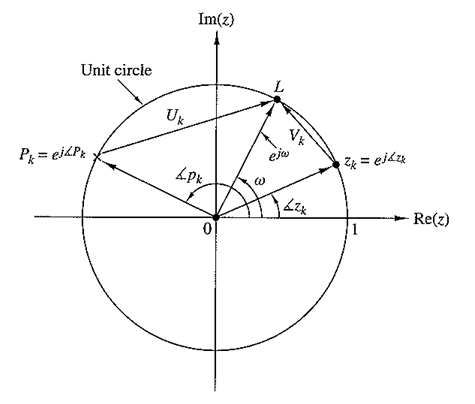
\includegraphics[width=5cm]{polszerosHomega.png}
\end{center}
\caption{Relació entre la posició dels pols i zeros del sistema amb la seva resposta en freqüència.}
\label{polszerosHomega}
\end{figure}

\vskip 0.3 cm
\noindent
\textbf{Exemple:} Raonau perquè el sistema descrit per la funció de transferència $H(z)=\frac{1}{1-0.8z^{-1}}$
té un pic de la magnitud de la resposta freqüencial a $\omega=0$.
 

\vskip 0.5 cm
\noindent
\textbf{\large Sistemes LTI com a filtres selectius en freqüència}

%Característiques dels filtres ideals: passa baix, passa banda, passa alt, banda eliminada i passa tot.
%
%Pols i zeros de filtres passa baix, passa banda i passa alt.
%Pols i zeros de filtres passa tot.
%
%Filtres de fase lineal i fase lineal generalitzada
%
%Filtres invertibles, filtres de fase mínima. 
%Descomposició d'un filtre en filtre de fase mínima i filtre passa-tot.


La paraula \textit{filtre} fa referència, en general, a un dispositiu
que discrimina, d'acord amb qualque atribut, els elements que passen
a través d'ell.

Per analogia, es parla de filtres freqüencials quan ens referim als sistemes
que permeten passar (amb poca o cap atenuació) senyals d'unes determinades freqüències
(\textbf{banda de pas})
i que atenuen (total o parcialment) senyals d'altres freqüencies (\textbf{banda de stop}).

Els \textbf{filtres ideals} són aquells que atenuen totalment una banda de freqüències
i deixen passar sense modificació una altra banda de freqüències. La magnitud 
de la seva resposta freqüencial es de la forma:
\[
|H(\omega)|=\begin{cases} 1 & \text{si } \omega_1 < \omega < \omega_2 \\ \\
0 & \text{altrament} \end{cases}
\]

En funció dels valors de $\omega_1$ i $\omega_2$ es parla de filtres passa-baix,
passa-banda, passa-alt, de banda eliminada o passa-tot (veure Figura \ref{idealfilters}).

\begin{figure}[htbp]
\begin{center}
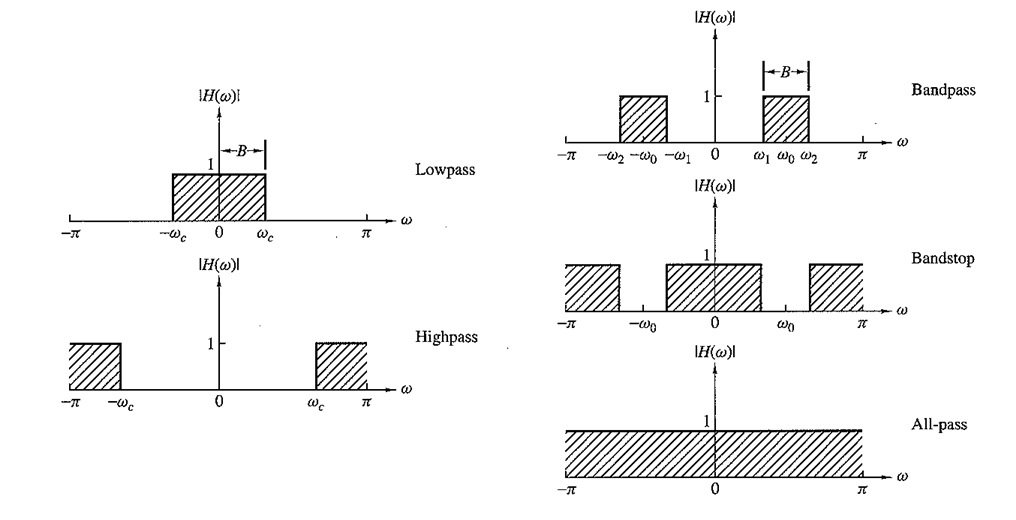
\includegraphics[width=12cm]{idealfilters.png}
\end{center}
\caption{Tipus de filtres ideals.}
\label{idealfilters}
\end{figure}

\vskip 0.3 cm
\noindent
\textbf{Diagrama de pols i zeros i tipus de filtres}

A partir de l'analisi de la relació entre la posició dels pols i zeros del sistema i la seva
resposta freqüencial (veure secció anterior) podem deduir si un sistema és passa-baix, passa-alt
o passa-banda observant el seu diagrama de pols i zeros. La Figura \ref{polszerosfiltres}
mostra un exemple per als casos dels filtres passa-baix i passa-alt.

\begin{figure}[htbp]
\begin{center}
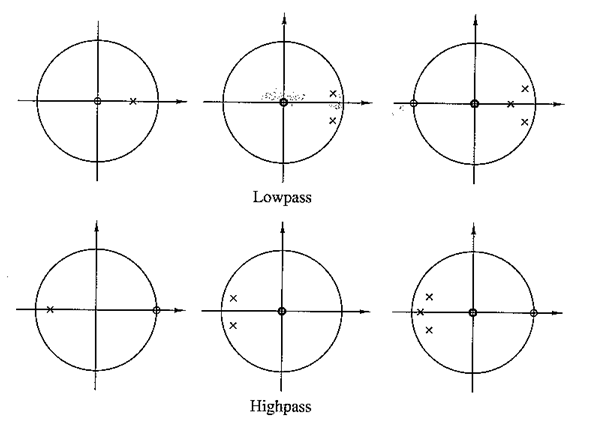
\includegraphics[width=7cm]{polszerosfiltres.png}
\end{center}
\caption{Diagrames de pols i zeros per a filtres passa-baix (dalt) i passa-alt (baix).}
\label{polszerosfiltres}
\end{figure}

\vskip 0.2 cm
Per al cas dels filtres passa tot tenim que 
\[
|H(\omega)|=1 \quad \forall \omega \qquad \text{equivalent a } \quad |H(\omega)|^2=1 \quad \forall \omega
\]

Si la funció de transferència del sistema s'escriu com una funció racional l'anterior relació
implica que $H(z)$ és de la forma 
\[
H(z)=z^{-N} \frac{A(z^{-1})}{A(z)}
\]

\noindent
ja que llavors
\[
|H(\omega)|^2=H(z) H(z^{-1})|_{z=e^{j\omega}}= z^{-N} \frac{A(z^{-1})}{A(z)} z^{N} \frac{A(z)}{A(z^{-1})}|_{z=e^{j\omega}}= 1
\]

En aquest cas, si $z_0$ \'es un pol de $H(z)$, llavors $\frac{1}{z_0}$ ha d'ésser un zero de $H(z)$ i viceversa.
La Figura \ref{polszerospassatot} mostra dos exemples de diagrames de pols i zeros per a filtres passa-tot.

\begin{figure}[htbp]
\begin{center}
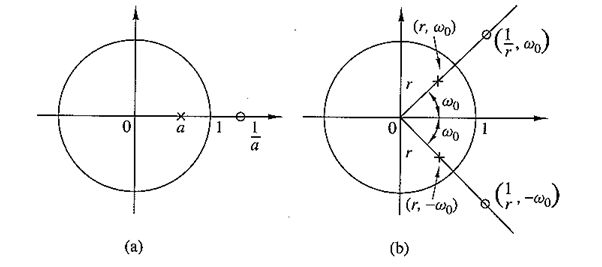
\includegraphics[width=8cm]{polszerospassatot.png}
\end{center}
\caption{Diagrames de pols i zeros per a filtres passa-tot.}
\label{polszerospassatot}
\end{figure}

\vskip 0.3 cm
\noindent
\textbf{Filtres de fase lineal}

En les seccions anteriors s'han definit els filtres ideals com aquells que tenen una magnitud 
de la resposta freqüencial igual a $1$ en una determinada banda de freqüències i $0$ fora
d'ella, però no hem parlat de la fase de la resposta freqüencial.

Direm que un filtre és de \textbf{fase lineal generalitzada} si $\Theta(\omega)=-\omega \alpha + \beta$.
Si $\beta=0$ direm que el filtre és de fase lineal. Anem a estudiar el comportament
dels filtres amb fase lineal generalitzada.

Sigui un filtre digital amb $h[n]$ real i resposta freqüencial
\[
H(\omega)=\begin{cases} C e^{-j( \omega \alpha - \beta)} & \text{si } \omega_1 < \omega < \omega_2 \\ \\
0 & \text{altrament} \end{cases}
\]

La resposta d'aquest filtre a un senyal sinusoïdal amb freqüencia $\omega \in (\omega_1, \omega_2)$ és:
\begin{equation}
\begin{array}{l}
y[n]=h[n] * \cos(\omega n)=A C \cos(\omega (n - \alpha) + \beta) \\ \\
y[n]=h[n] * \sin(\omega n)=A C \sin(\omega (n - \alpha)+ \beta)
\end{array} 
\end{equation}

És a dir, la sortida del sistema és una versió atenuada, retardada i desplaçada en fase del senyal d'entrada.
Malgrat que aquest comportament del filtre estigui lluny del comportament ideal (voldriem un senyal idèntic
al d'entrada a la sortida), el fet que per a totes les freqüències $\omega \in (\omega_1, \omega_2)$ es tengui
la mateixa atenuació, retard i desplaçament de fase fa que, per a senyals compostos per vàries freqüències,
el senyal de sortida tengui la mateixa \textit{forma} que el d'entrada (no hi ha \textit{distorsió}). 
Això no passaria si cada freqüència
es veiés afectada de forma diferent pel filtre. És per aquest motiu que els filtres amb fase lineal generalitzada
es consideren \textit{suficientment bons} per al filtratge de senyal i no s'exigeix que els filtres ideals
tenguin fase $0$ ($\Theta(\omega)=0$).


\vskip 0.3 cm
\noindent
\textbf{Filtres de fase mínima. Filtres invertibles}

Un filtre és diu de fase mínima si tots els pols i els zeros de la seva funció de transferència
es troben a l'interior del cercle unitat. 

Si la funció de transferència és de la forma $H(z)=\frac{B(z)}{A(z)}$ i el filtre és
de fase mínima llavors:
\begin{itemize}
\item el filtre és estable i causal
\item el filtre és invertible, és a dir, existeix una funció $H_I(z)$ tal que $H(z) H_I(z)=1$.
En aquest cas $H_I(z)=\frac{1}{H(z)}=\frac{A(z)}{B(z)}$
\item el filtre invers és estable i causal
\end{itemize}

Una darrera propietat relativa als filtres de fase mínima és que la funció de transferència de
qualsevol filtre amb fase no mínima és pot escriure com el producte de les funcions de
transferència d'un filtre de fase mínima i un filtre passa tot:

\[
H(z)=H_{\text{min}}(z) H_{\text{pt}}(z)
\]

En particular, si el filtre és estable i causal amb $H(z)=\frac{B(z)}{A(z)}$ i 
$B(z)$ es pot descomposar com $B(z)=B_1(z) B_2(z)$,
on $B_1(z)$ té totes les seves arrels dins el cercle unitat i $B_2(z)$ fora del cercle unitat,
llavors 
\[
H_{\text{min}}(z)=\frac{ B_1(z) B_2(z^{-1}) }{A(z)}
\qquad 
H_{\text{pt}}(z)=\frac{B_2(z)}{B_2(z^{-1})}
\]
\noindent
on $B_2(z^{-1})$ és un polinomi amb totes les seves arrels dins el cercle unitat i $A(z)$ té també 
totes les seves arrels dins el cercle unitat ja que el filtre és estable i causal. 

 

\vskip 0.5 cm
\noindent
\textbf{\large Disseny de filtres digitals}

%El problema de la no-causalitat dels filtres ideals
%
%Característiques dels filtres causals i realitzables
%
%Propietats de simetria dels filtres FIR de fase lineal generalitzada
%
%Disseny de filtres FIR de fase lineal mitjançant finestres
%Disseny de filtres FIR de fase lineal per mostreig de freqüències
%Disseny de filtres IIR a partir de filtres analògics: filtres Butterworth i Txebyshev
%

\vskip 0.2 cm
\noindent
\textbf{El problema de la no-causalitat dels filtres ideals}

Considerem un filtre passa-baix ideal amb funció de transferència
\[
H(\omega)=\begin{cases} 1 & \text{si } |\omega| \leq \omega_c \\ 0 & \text{altrament} \end{cases}
\]

La transformada inversa d'aquesta funció dóna com a resposta impulsional
\[
h[n]=\begin{cases} \frac{\omega_c}{n} & \text{si } n=0 \\ 
\frac{\omega_c}{n} \mathrm{sinc}(\omega_c n) & \text{altrament} \end{cases}
\]

Observam (Figura \ref{passabaixideal}) que aquesta resposta impulsional correspon a un filtre no causal i per tant és \textbf{irrealitzable}.
En general obtenim el mateix resultat per a qualsevol filtre ideal: qualsevol filtre per al qual
$|H(\omega)|=0$ en un interval de freqüències (cas de tots els filtres ideals) és un filtre no causal i per
tant irrealitzable.

\begin{figure}[htbp]
\begin{center}
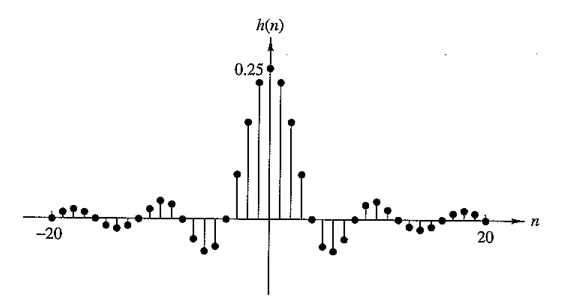
\includegraphics[width=7cm]{passabaixideal.png}
\end{center}
\caption{Resposta impulsional d'un filtre passa-baix ideal.}
\label{passabaixideal}
\end{figure}

\vskip 0.3 cm
De manera que a l'hora de dissenyar un filtre realitzable (i per tant causal) no podem esperar obtenir 
una resposta en freqüència com les mostrades en la Figura \ref{idealfilters} sino que ens haurem de 
conformar amb una resposta com la que es mostra en la Figura \ref{realizablefilters}.
En aquesta figura els valors de $\delta_1$, $\delta_2$, $\omega_p$ i $\omega_c$ indiquen els marges
de tolerància permesos en el disseny del filtre.

\begin{figure}[htbp]
\begin{center}
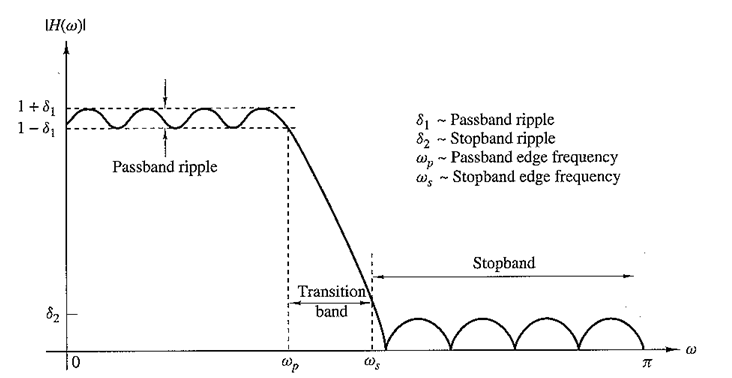
\includegraphics[width=7cm]{realizablefilters.png}
\end{center}
\caption{Magnitud de la resposta freqüencial d'un filtre realitzable}
\label{realizablefilters}
\end{figure}

\vskip 0.3 cm
\noindent
\textbf{Disseny de filtres FIR}

En aquestes seccions ens centram en l'estudi d'algunes tècniques per al disseny de filtres
causals amb resposta impulsional finita (FIR) i amb fase lineal generalitzada.

\vskip 0.3 cm
\noindent
\textbf{Propietats de simetria dels filtres FIR de fase lineal generalitzada}

Considerem el cas general d'un filtre FIR causal de longitud $M+1$:
\[
h[n]=\{ h[0], h[1], \cdots, h[M-1], h[M] \}
\]

Es pot demostrar que el filtre és de fase lineal generalitzada si 
\[
h[n]=\pm h[M-n] \qquad \forall n=0, 1, \cdots, M
\]

(la implicació inversa no és certa, és a dir, un filtre pot ésser de fase lineal
sense verificar l'anterior relació).

Aquesta condició implica que la transformada Z de $h[n]$ ha de verificar:
\[
z^{-M}H(z^{-1})=\pm H(z)
\]
\noindent
És a dir, les arrels del polinomi $H(z)$ també són arrels de $H(z^{-1})$, la qual cosa significa que si
$z_i$ és zero de $H(z)$ llavors $\frac{1}{z_i}$ també ho és. A més, si $h[n]$ és real llavors
les arrels complexes han de formar parells conjugats i per tant, si $z_i$ és zero de $H(z)$ llavors
$z_i^*$,$1/z_i$ i $1/z_i^*$ també són arrels. La Figura \ref{zerosFIRlineal} mostra un exemple
de la distribució dels zeros en un filtre FIR causal real de fase lineal.

\begin{figure}[htbp]
\begin{center}
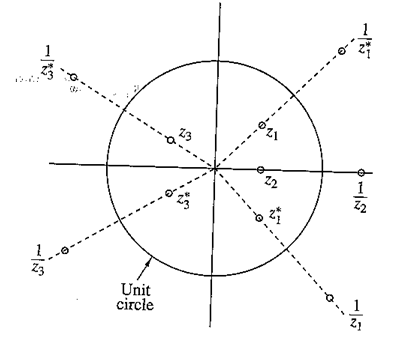
\includegraphics[width=5cm]{zerosFIRlineal.png}
\end{center}
\caption{Exemple de la distribució dels zeros en un filtre FIR causal real de fase lineal.}
\label{zerosFIRlineal}
\end{figure}

\vskip 0.2 cm
Si $h[n]=h[M-n]$ és diu que el filtre FIR de fase lineal és \textbf{simètric}.
Si $h[n]=-h[M-n]$ és diu que el filtre és \textbf{antisimètric}. En ambdos casos es pot distingir
entre els filtres amb un nombre de mostres ($M+1$) parell o imparell. Això dóna lloc
a quatre configuracions possibles per als filtres FIR de fase-lineal:
tipus I (simètric imparell), tipus II (simètric parell), tipus III (antisimètric imparell)
i tipus IV (antisimètric parell). La Figura \ref{tipusFIR} mostra un exemple de cada tipus
i la Figura \ref{tipusFIR_H} mostra la magnitud de les seves respostes en freqüència.
Observam que els filtres tipus I i II són filtres passa-baix, els tipus III passa banda 
i el tipus IV passa-alt.

\begin{figure}[htbp]
\begin{center}
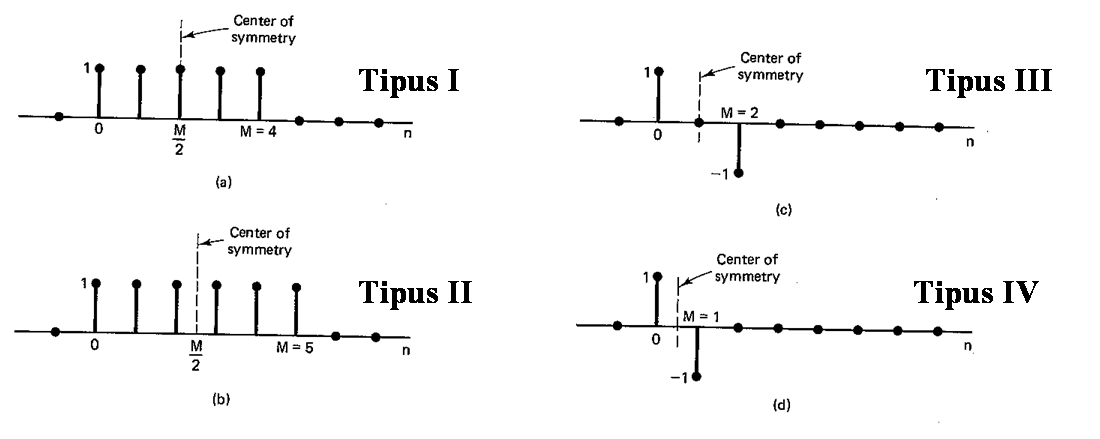
\includegraphics[width=12cm]{tipusFIR.png}
\end{center}
\caption{Exemples de configuracions de filtres FIR de fase lineal. Font: Discret-Time Signal
Processing, A. Oppenheim, W. Schafer, Prentice-Hall, 1989}
\label{tipusFIR}
\end{figure}

\begin{figure}[htbp]
\begin{center}
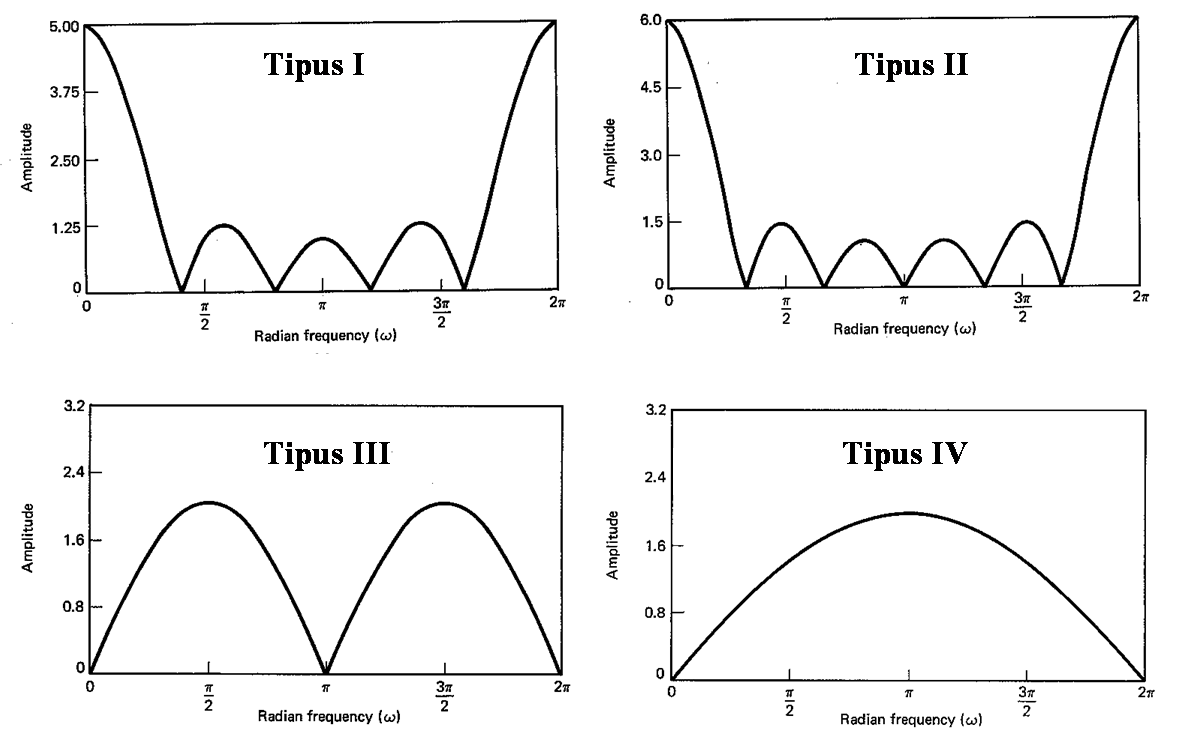
\includegraphics[width=10cm]{tipusFIR_H.png}
\end{center}
\caption{$|H(\omega)|$ per a les configuracions de filtres FIR de fase lineal de la figura \ref{tipusFIR}.
Font: Discret-Time Signal
Processing, A. Oppenheim, W. Schafer, Prentice-Hall, 1989}
\label{tipusFIR_H}
\end{figure}



\vskip 0.3 cm
\noindent
\textbf{Disseny de filtres FIR de fase lineal mitjançant finestres}

A partir d'una resposta en freqüència especificada $H_d(\omega)$ l'objectiu és
trobar un filtre, amb una resposta impulsional $h[n]$, causal i que tengui 
una resposta en freqüència $H(\omega)$ similar a $H_d(\omega)$.

El filtre ideal $h_d[n]$ es pot obtenir fent l'antitransformada de Fourier de $H_d(\omega)$:
\[
h_d[n]=\frac{1}{2\pi} \int_{-\pi}^\pi H_d(\omega) e^{j\omega n} \, d\omega
\]

\noindent
com $h_d[n]$ té una resposta impulsional infinita i per tant no causal, s'aproxima mitjançant
un filtre causal $h[n]$ de la següent manera:
\[
h[n]=\begin{cases} h_d[n] & \text{si } n \geq 0 \\ 0 & \text{altrament} \end{cases}
\]

Aquest procés és equivalent a multiplicar $h_d[n]$ per una \textit{finestra} 
$w[n]=\begin{cases} 1 & \text{si } n \geq 0 \\ 0 & \text{altrament} \end{cases}$:
\[
h[n]=h_d[n] w[n]
\]

\noindent
Per tant:
\[
H(\omega)={\cal F}^{-1} \{ h_d[n] w[n] \} = H_d(\omega) * W(\omega) 
\]

\noindent
$h[n]$ es troba fent l'antitransformada d'aquesta funció.

La Figura \ref{exdissenyfinestra} mostra alguns resultats d'aplicar aquest mètode al disseny
d'un filtre passa-baix ideal. A part de la finestra rectangular $w[n]$ definida més amunt es poden definir
finestres amb formes diferents que permeten aproximar millor el comportament dels filtres ideals.


\begin{figure}[htbp]
\begin{center}
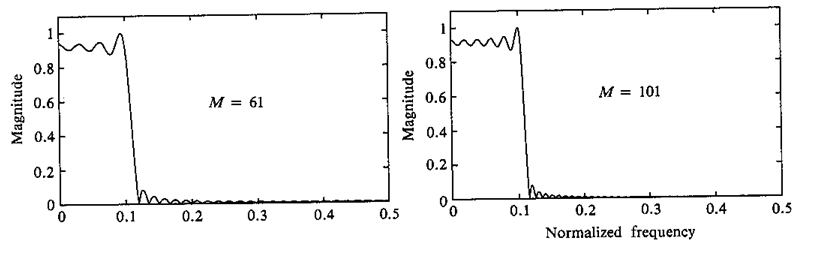
\includegraphics[width=10cm]{exdissenyfinestra.png}
\end{center}
\caption{Exemples de disseny d'un filtre passa-baix amb finestres.}
\label{exdissenyfinestra}
\end{figure}



\vskip 0.3 cm
\noindent
\textbf{Disseny de filtres FIR de fase lineal per mostreig de freqüències}

En aquest cas s'especifica $H_d(\omega)$ per a un conjunt discret de freqüències $\omega_k$
i es troben els valors de $h[n]$ resolent un sistema d'equacions.

\vskip 0.3 cm
\noindent
\textbf{Disseny de filtres FIR de fase lineal òptims}

Els mètodes de disseny anterior no permeten controlar de manera precisa les freqüències de
separació de la banda de pas i la de stop.
Els filtres FIR de fase lineal òptims minimitzen la diferència entre les respostes del filtre
ideal i el filtre dissenyat en cada una de les bandes. L'equació d'aquest filtres es troba
resolent un problema de minimització, seguint una tècnica formulada per Txebytxev.



\vskip 0.3 cm
\noindent
\textbf{Disseny de filtres IIR}

Les tècniques de disseny de filtres IIR es basen en la conversió de filtres analògics a filtres
digitals. Els filtres analògics es dissenyen per a verificar una sèrie d'especificacions,
seguint unes tècniques de disseny ben conegudes en l'àrea del processament analògic: disseny
tipus Butterworth o disseny tipus Txebyshev. La figura \ref{ButtTxeby} mostra un exemple
de la forma de la resposta freqüencial de cada tipus de filtre. La conversió de les expresions
obtingudes al cas discret es fa mitjançant un canvi de variables (transformació bilineal).

\begin{figure}[htbp]
\begin{center}
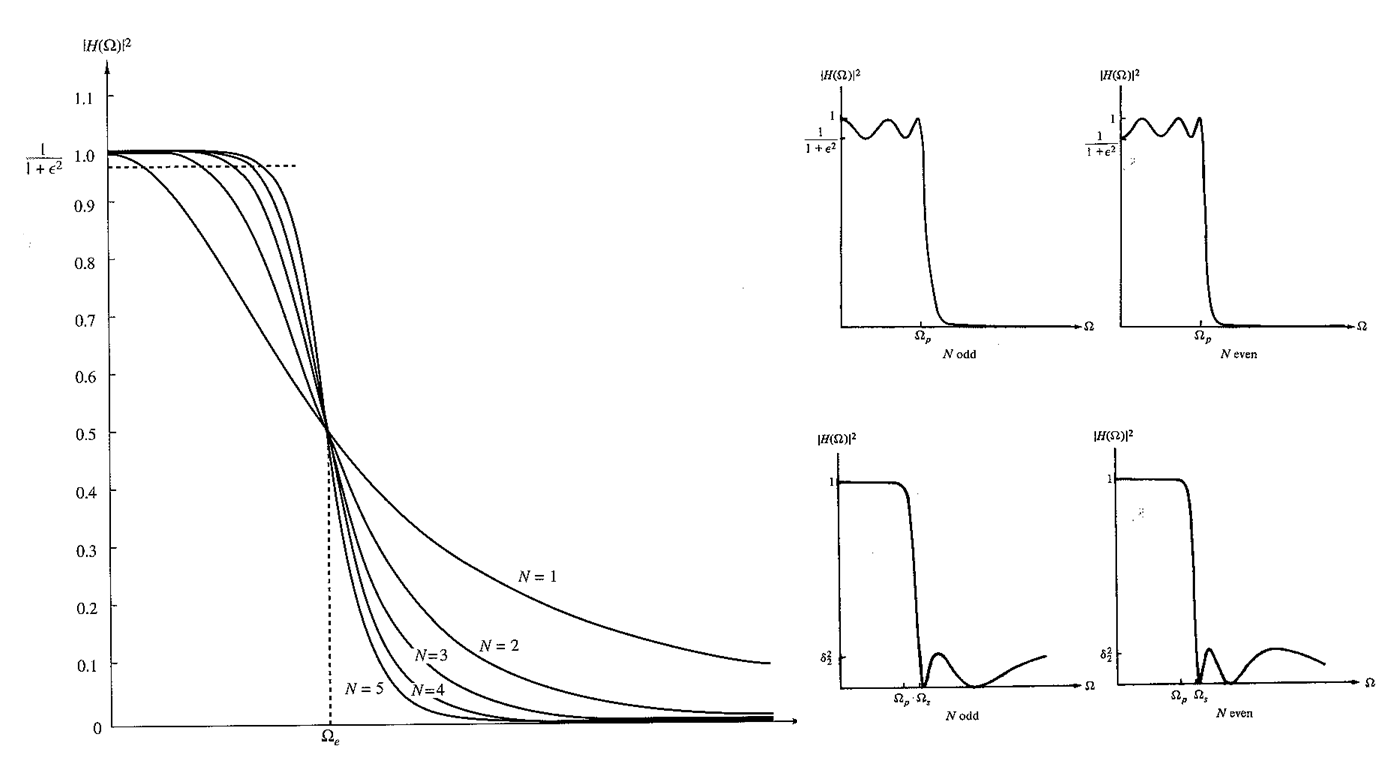
\includegraphics[width=12cm]{ButtTxeby.png}
\end{center}
\caption{Exemples de respostes en freqüència de filtres analògics Butterworth (esquerra) i Txebytxev (dreta).}
\label{ButtTxeby}
\end{figure}


\vskip 7cm
\noindent
\textbf{Nota:} la majoria de figures d'aquest cap\'itol s'han tret de Digital Signal Processing, J. Proakis, D. Manolakis, Pearson Prentice Hall, 2007.




\end{document}